\documentclass[12pt, a4]{article}
\usepackage[T1]{fontenc}
\usepackage{graphicx}
\usepackage[brazil]{babel}
\usepackage{mathtools}
\usepackage{amsmath,array}
\usepackage{longtable}
\usepackage{enumitem}
\usepackage{float}
\usepackage{tikz}

\begin{document}
\begin{titlepage}

\newcommand{\disciplina}{Processamento de Materiais I: Solidificação e Fundição (SMM 0302)}
\newcommand{\titulo}{Desafio PBL Tupy x USP 2025: Primeira Entrega}


\newcommand{\prof}{Prof. Dr. Marcelo Falcão de Oliveira}
\newcommand{\data}{São Carlos,\\ 12 de setembro 2025}



\center


\begin{tikzpicture}[remember picture,overlay]
   
    \node[anchor=north west, xshift=1cm, yshift=-1cm] at (current page.north west) 
    {
\includegraphics[scale=0.6]{eesclogo.png}};
    
    \node[anchor=north east, xshift=-1cm, yshift=-1cm] at (current page.north east) 
    {
\includegraphics[scale=0.6]{tupylogo.png}};
\end{tikzpicture}


\textbf{\Large\titulo}

\begin{center}
    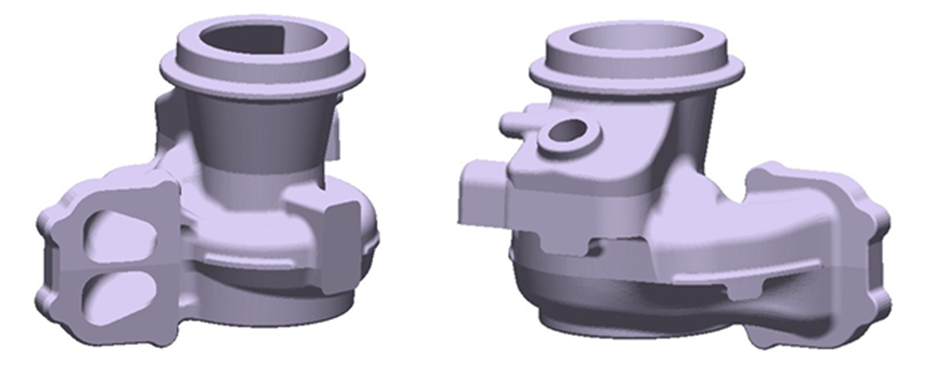
\includegraphics[scale=0.8]{peca1.png}
\end{center}



\textbf{\disciplina}

\vspace{0.5cm}

\textbf{\prof}

\vspace{0.5cm}

\begin{flushright}
\begin{tabular}{l l}
    Ana Julia Borges Guerra & 11799962\\
    Guilherme Capputti Mazzini & 14099960\\
    Ítalo Cunha Melo Silva & 11223292\\
    Murilo Fernandes Pinto & 14599895\\
    Ricardo Rodrigues da Silva & 14616503
\end{tabular}
\end{flushright}

\vfill
\data

\end{titlepage}
\pagebreak






\end{document}